\documentclass[10pt,a4paper]{article}
\usepackage[utf8]{inputenc}
\usepackage{amsmath}
\usepackage{amsfonts}
\usepackage{amssymb}
\usepackage{graphicx}
\usepackage[margin=0.5in]{geometry}

\author{Oleg Loshkin}
\title{\textbf{UPDC}\\Unity to PokEngine Data Converter\\\textbf{User Manual}}
\graphicspath{{./images/}}

\begin{document}
\maketitle
\section{Introduction}
The \textbf{Unity to PokEngine Data Converter, or UPDC for short}, is a Unity tool used to \textbf{export ScriptableObject} inheriting .asset files \textbf{into JSON files} that end with extensions that specify their type. These JSON files can then be read by the PokEngine's parser.

\section{Accessing the Tool}
\begin{center}
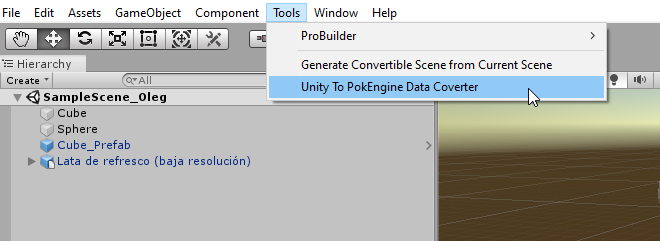
\includegraphics[scale=1.0]{mainMenu}
\end{center}
The tool is accessed via \textbf{MainMenu/Tools/Unity to PokEngine Data Converter}.
\newpage

\section{Configuring the Tool}
\textbf{UPDC uses} it's \textbf{own ScriptableObjects \texttt{"Persistent\_SO"} and \texttt{"TypesAndExtensions\_SO"}} for data that must persist across sessions. \textbf{You will need to configure these.}\\
These are \textbf{located under \texttt{"Assets/Editor/UPDC/UPDC\_SO"}}. \textbf{If instances of these ScriptableObjects do not exist, create them} via the context menu as such:
\begin{center}
\includegraphics[scale=0.70]{so}
\end{center}
\newpage
\noindent Once that's done, \textbf{set up the default output directory's path} as it appears on your system. This should look something like "C:/myProjectPath/Assets/Editor/UPDC/DefaultOutputDir":
\begin{center}
\includegraphics[scale=0.80]{soLocation}
\end{center}
Alternatively, you could chose to make any other directory your default output directory, which case, \\Assets/Editor/UPDC/DefaultOutputDir may be safely deleted.
\textbf{If these are not set up correctly, you will see errors} in the Unity console and/or when opening the UPDC Editor.

\section{The Exporter Tab}
\begin{center}
\includegraphics[scale=0.55]{exportUi}
\end{center}
The tool is separated between \textbf{two tabs}. In the \textbf{Exporter tab}, you can \textbf{select the .asset files located in the Assets/Data/...} folders \textbf{you wish to export}.
You can \textbf{select the output directory} for the files generated. By default, the tool outputs the files into Assets/Editor/UPDC/DefaultOutputDir you have previously defined.
Upon exportation, \textbf{directories will be generated in the output directory} to mirror the structure seen in Assets/Data.\\
Finally, you can choose to \textbf{overwrite any existing files} and choose between a \textbf{human friendly readable format} or an \textbf{optimised one} for the JSON.
\newpage

\section{Integrating with UPDC}
\textbf{UPDC converts .asset files} of types \textbf{inheriting from the ScriptableObject} class.\\
If you wish to export your data using UPDC, you will therefore need to \textbf{create your ScriptableObject inheriting class} as such:
\begin{center}
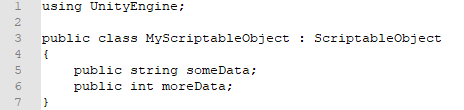
\includegraphics[scale=1.0]{soExample}
\end{center}
\textbf{Instances of your ScriptableObject inheriting class will need to be stored in Asssets/Data/yourTypeFolder} for UPDC to manage them. \textbf{This must be done on your side} as UPDC does not provide any automatic way to put your .asset files into their corresponding folders.
Next, you will need to \textbf{define your new class with UPDC} via the "Types" tab.

\section{The Types Tab}
\begin{center}
\includegraphics[scale=0.55]{typesUi}
\end{center}
The \textbf{Types tab} contains a list of \textbf{tuples that define a type's name and it's corresponding extension}.
The type's name is used for generating appropriately named folders and the extension is appended to the JSONs generated for your custom class to be used by the PokEngine's parser to identify the asset's type.
\begin{center}
\includegraphics[scale=0.55]{folderUPDC}
\end{center}
\textbf{To integrate your newly created class} with UPDC, simply \textbf{enter it's name and it's extension} in the "New entry" fields and press the \textbf{"Add new type" button}.
A \textbf{folder for your new .asset files will be automatically generated} in Assets/Data and the files will be visible in the "Export" tab.\\
To \textbf{remove a type}, simply \textbf{select it} in the list and press the \textbf{"Remove selected" button}.

\end{document}
